\subsection{QuizziPedia::Front-End}
\subsubsection{Informazioni generali}
\label{QuizziPedia::Front-End}
\begin{figure}
	\centering
	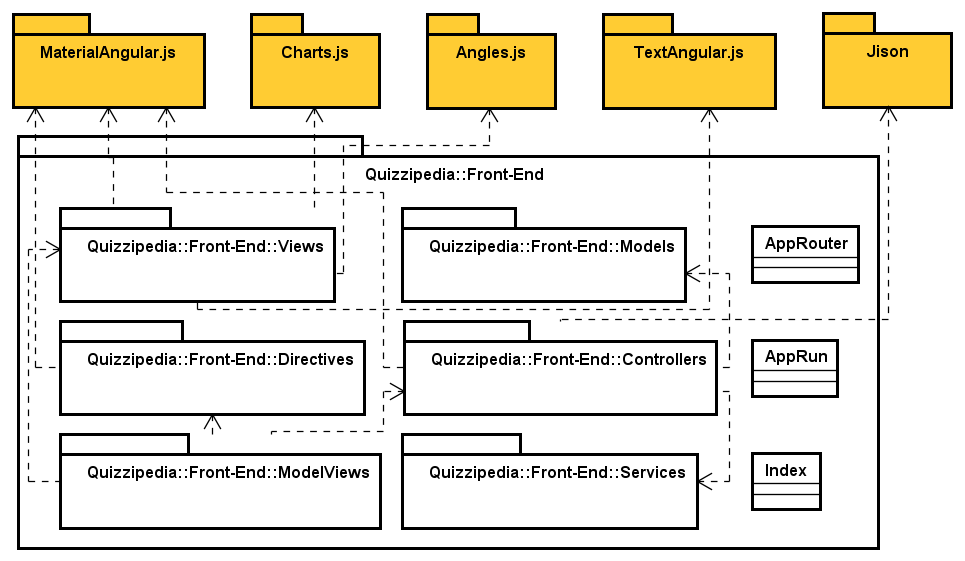
\includegraphics[scale=0.45]{UML/Package/QuizziPedia_Front-end.png}
	\caption{QuizziPedia::Front-End}
\end{figure}

	\begin{itemize}
		\item \textbf{Descrizione} \\ Package contenente le componenti front-end dell'applicazione.
		\item \textbf{Package contenuti}
		\begin{itemize}
			\item \texttt{Controllers} \\ Package contenente i controllers front-end dell'applicazione.
			\item \texttt{Directives} \\ Package contenente le directives front-end dell'applicazione.
			\item \texttt{Models} \\ Package contenente le classi che definiscono la business logic dell'applicazione.
			\item \texttt{Services} \\ Package contenente i services front-end dell'applicazione.
			\item \texttt{Views} \\ Package contenente le views front-end dell'applicazione.
			\item \texttt{Templates} \\ Package contenente i templates front-end dell'applicazione.
		\end{itemize}
	\end{itemize}
	